\subsection{Bidirectional mapping through an example}
\label{subsec:bimapping}
We present our additional constructs through a producer-consumer example, whose architecture is specified by Fig. \ref{fig:approachexample} \encircle{a}, \encircle{b}, and \encircle{c}.
The \ttt{p} producer sends data items to a first-in first-out component \ttt{FIFO} storing data.
The \ti{FIFO} queue has a limited size, an attribute for the number of currently stored items (\ttt{numberOfItems}) and the \ttt{isQueueFull} operation for validating its availability.
The \ti{pPush} port of the producer with \ttt{IPush} as required interface is connected to the \ti{pPush} port of \ti{FIFO} with \ttt{IPush} as provided interface. %so that the producer and FIFO can interact with each other through their respective port.
\ttt{FIFO} also provides the \ti{IPull} interface for the consumer to pull data items.
FIFO implements the two interfaces in Fig. \ref{fig:approachexample} \encircle{b}.

The behavior of \ttt{FIFO} is described by using a UML State Machine as shown in Fig. \ref{fig:approachexample} \encircle{c}.
Initially, the \ttt{Idle} state is active.
The state machine then waits for an item to arrive at the \ttt{fifo} component (through the \ttt{pPush} port).
The item is then checked for its validity before verifying the fullness of the queue to decide to either add the item to the queue or discard it.

Table \ref{table:mapping} shows some of the UML meta-classes and the equivalent constructs in the extended language.
The constructs are categorized into \ti{structural} (three upper rows) and \ti{behavioral constructs} (seven lower rows).
%We explain these constructs in the followings.

\begin{comment}
\begin{table}[]
	\centering
	\caption{My caption}
	\label{my-label}
	\begin{tabular}{lllll}
		UML                  & XGC                      &  & OO                             & C++                 \\ \cline{1-2} \cline{4-5} 
		Class component      & Class                    &  & Class                          & Class               \\ \cline{1-2} \cline{4-5} 
		Part                 & Part                     &  & Composition attribute          & Attribute           \\ \cline{1-2} \cline{4-5} 
		Port  (data/control) & Port                     &  & Attribute                      & Reference Attribute \\ \cline{1-2} \cline{4-5} 
		Many ports           & Multiple-port            &  & Multiple interface realization & --                  \\ \cline{1-2} \cline{4-5} 
		Connector            & Binding (static+dynamic) &  & --                             & Methods             \\ \cline{1-2} \cline{4-5} 
		Interface            & Class/Interface          &  & Interface                      & Class               \\ \cline{1-2} \cline{4-5} 
		Signal               & Class                    &  & Class                          & Class/Struct        \\ \cline{1-2} \cline{4-5} 
		State machine        & state\_machine           &  & --                             & --                  \\ \cline{1-2} \cline{4-5} 
		State                & state                    &  & --                             & --                  \\ \cline{1-2} \cline{4-5} 
		Region               & region                   &  & --                             & --                  \\ \cline{1-2} \cline{4-5} 
		CallEvent            & call\_event              &  & --                             & --                  \\ \cline{1-2} \cline{4-5} 
		TimeEvent            & time\_event              &  & --                             & --                  \\ \cline{1-2} \cline{4-5} 
		ChangeEvent          & change\_event            &  & --                             & --                  \\ \cline{1-2} \cline{4-5} 
		SignalEvent          & signal\_event            &  & --                             & --                  \\ \cline{1-2} \cline{4-5} 
		Any                  & any                      &  & --                             & --                  \\ \cline{1-2} \cline{4-5} 
		Pseudo state         & pseudo\_state            &  & --                             & --                  \\ \cline{1-2} \cline{4-5} 
		Action/Effect        & Method                   &  & Method                         & Method             
	\end{tabular}
\end{table}
\end{comment}

\begin{table}[]
	\centering
	\caption{Mapping between UML and Examples of Extended Language}
	\label{table:mapping}
	\begin{tabular}{lll}
		UML                                                                      & Extended Language                                                                                & Code example in Fig. \ref{fig:approachexample}                                                                               \\ \hline
		\begin{tabular}[c]{@{}l@{}}Port requiring \\ an interface \ti{I}\end{tabular} & \begin{tabular}[c]{@{}l@{}}Attribute typed \\ by \ti{RequiredPort}\textless I\textgreater\end{tabular} & \begin{tabular}[c]{@{}l@{}}Ports \ti{pPush} and \ti{pPull} at lines\\ 21 and 25\end{tabular}         \\ \hline
		\begin{tabular}[c]{@{}l@{}}Port providing \\ an interface \ti{I}\end{tabular} & \begin{tabular}[c]{@{}l@{}}Attribute typed\\ by \ti{ProvidedPort}\textless I\textgreater\end{tabular}  & \begin{tabular}[c]{@{}l@{}}Ports \ti{pPush} and \ti{pPull} at \\ lines 29-30\end{tabular}            \\ \hline
		Connector                                                                & Binding                                                                                        & Lines 7-8                                                                                  \\ \hline
		State Machine                                                            & \ti{StateMachine}                                                                                     & \begin{tabular}[c]{@{}l@{}}The FIFO state machine at \\ lines 34-59\end{tabular}           \\ \hline
		State                                                                    & \ti{State/InitialState}                                                                               & \begin{tabular}[c]{@{}l@{}}State \ti{SignalChecking} at \\ lines 36-39\end{tabular}             \\ \hline
		Region                                                                   & \ti{Region}                                                                                           & Not shown in this paper                                                                                 \\ \hline
		Pseudo state                                                             & \begin{tabular}[c]{@{}l@{}}Attribute typed \\ by pseudo type\end{tabular}                        & \begin{tabular}[c]{@{}l@{}}The \ti{dataChoice} pseudo state \\ at line 49\end{tabular}          \\ \hline
		Action/Effect                                                            & Method                                                                                           & Methods at lines 60-65       \\ \hline
		Transitions                                                           & Transition table                                                                                           & Transition table at lines 51-58	\\ \hline
		Event                                                            & Event                                                                                           & The call event at line 50                                                             
	\end{tabular}
\end{table}



\subsubsection{Structural constructs}
We explain the constructs used for representing the architecture structure.

%\noindent
%\tb{Part:}
%In the extended language, we introduce the \ti{Part<T>} template class.
%A UML part is typed by a UML class and mapped to a standard class attribute typing the template class with the \ti{T} template parameter replaced by the class equivalent to the UML class typing the UML part. 
%For example, at line 3, the \ti{p} attribute is equivalent to the \ti{p} part in the model.

\noindent
\tb{Port:}
Template-based constructs proposed in the extended language correspond to architecture component interaction points specified by UML ports.
\ti{RequiredPort<T>} and \ti{ProvidedPort<T>} (see Table \ref{table:mapping}) are equivalent to UML uni-directional ports, which have only one required or provided interface.
The \ti{T} template parameter is an interface in code (e.g. \ti{interface} in Java or class with \ti{pure virtual} methods in C++) equivalent to the interface required/provided by a UML port. 
\ti{BidirectionalPort<R,P>} (not shown) is also proposed to map to UML bidirectional ports, which have one required and one provided interface.

%Three constructs, \ti{Part}, \ti{Port}, and \ti{Binding}, are introduced to represent UML \ti{part}, \ti{port}, and \ti{connector}, respectively, because these UML concepts do not have equivalences in the existing programming language.
%Fig. \ref{fig:approachexample} \encircle{d} shows the extended code containing our additional constructs for the producer-consumer example.

%In the extended code, the \ti{Part}s and \ti{Port}s constructs are template classes.
%The template parameters of the latter specify the types of \ti{Part}s or required/provided interfaces of \ti{Port}s.
%For example, lines 3-5 show the three parts corresponding to the ones defined in the model.
Lines 21 and 25 show ports with a required interface and lines 29-30 show ports with a provided interface of the \ti{Producer}, \ti{Consumer}, and \ti{FIFO} classes.

\noindent
\tb{Binding:}
A binding (see Table \ref{table:mapping}, row 3) connects two ports equivalently to a UML connector connecting two UML ports.
A binding is a method call to our predefined method \ti{bindPorts.}
%UML connectors for communicating UML parts through UML ports are mapped to method calls (bindings) in the extended code.
Lines 7-8 shows two invocations of \ti{bindPorts}, which takes as input two ports (the two ports of the producer and fifo, for example).
Each class associated with a UML component contains a single configuration (as a method in lines 6-9) containing bindings.
The configuration method is restricted to contain only invocations to \ti{bindPorts} for synchronization ease.

Other model elements in the class diagram are mapped to the corresponding elements as in industrial tools such as IBM Rhapsody and Enterprise Architect.
For example, the \ti{p, fifo, c} UML parts are mapped to the composite attributes of the \ti{System} class; the UML operations and properties are mapped to the class methods and attributes (not shown in the paper), respectively; the UML interfaces (\ti{IPush} and \ti{IPull}) mapped to classes with pure virtual methods (lines 11-18) (in C++). 

  

\begin{figure*}
	\centering
	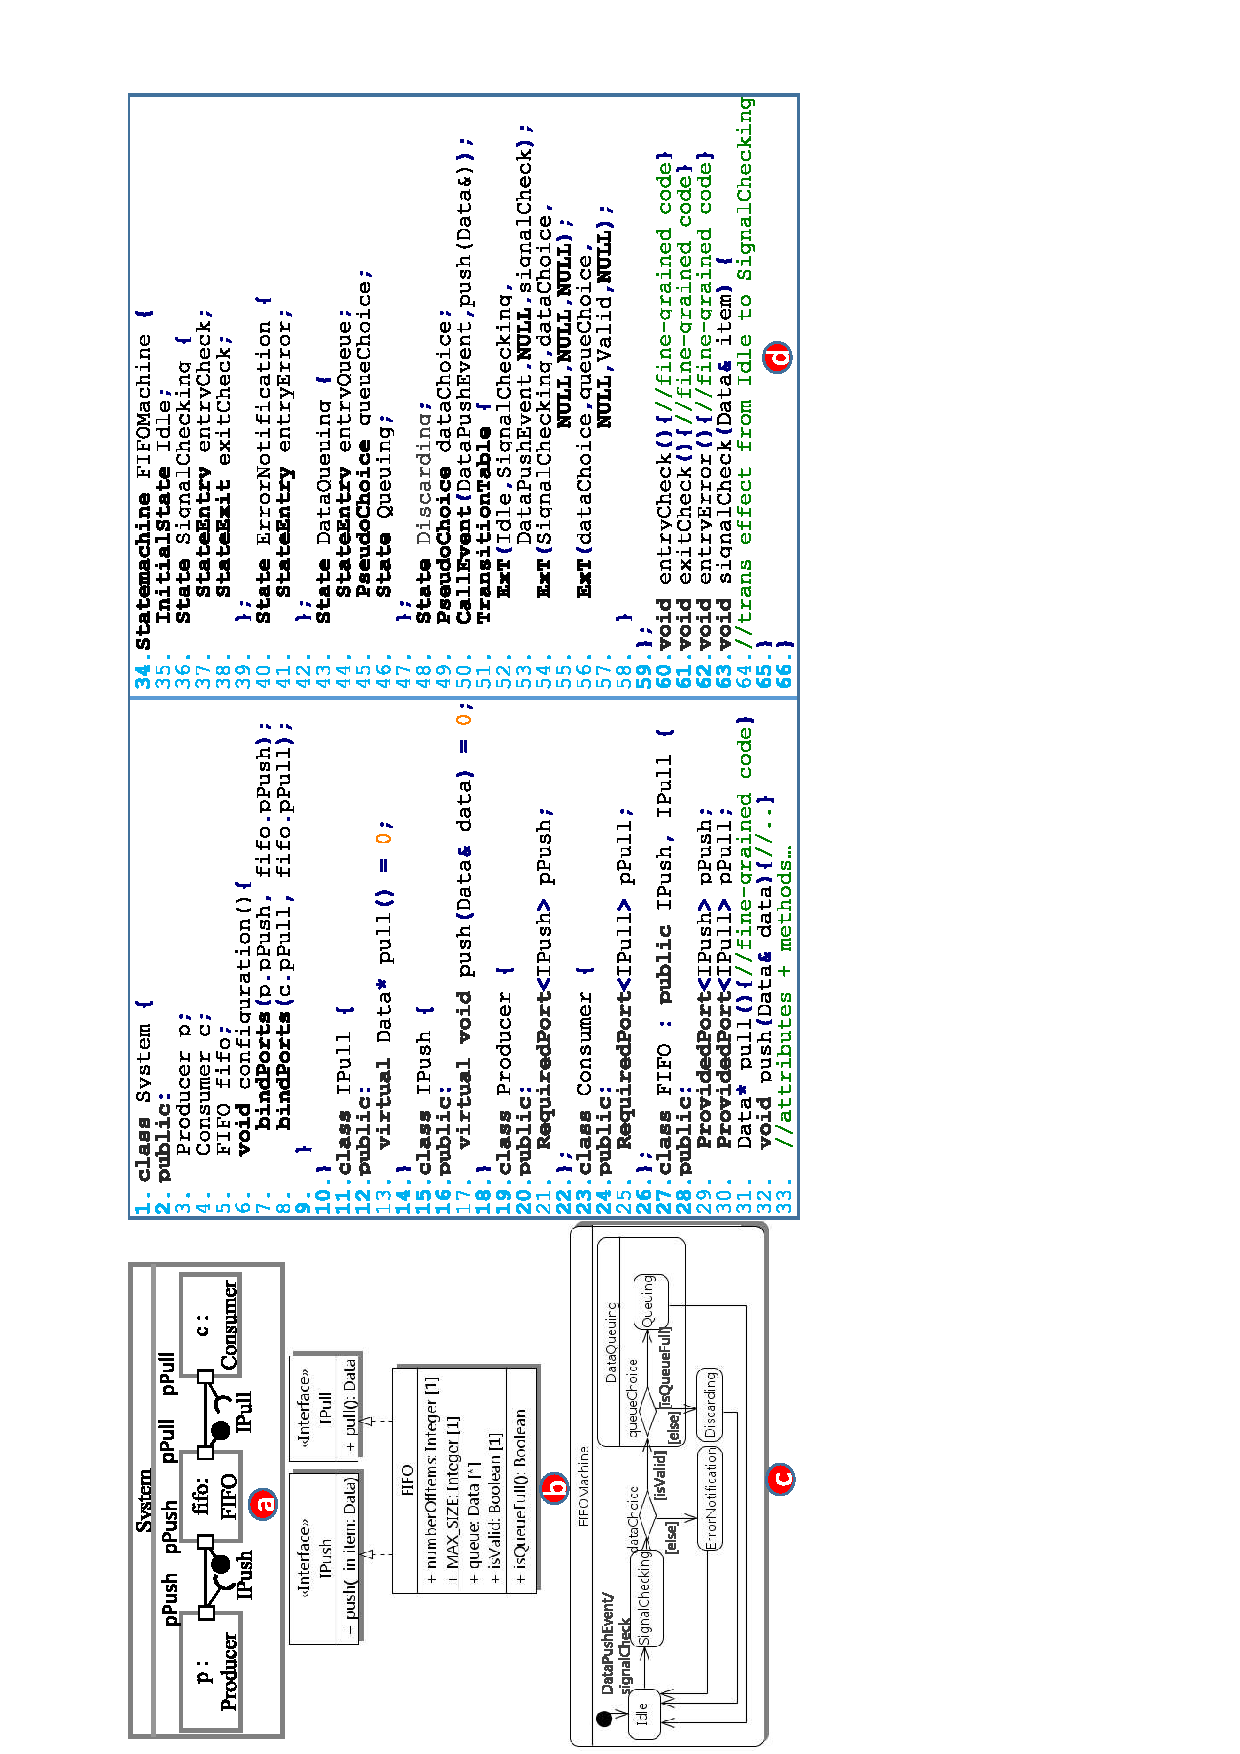
\includegraphics[angle=-90,clip, trim=2cm 0cm 7.0cm 1cm, width=\textwidth]{figures/approachexample3.pdf}
	\caption{Architecture model and generated extended code} 
	\label{fig:approachexample}
\end{figure*}


\subsubsection{Behavioral constructs}
%Applying XSeparation to UML State Machines, XSeparation-generated code contains our syntactic sugar of additional constructs for explicitly representing domain-specific concepts of state machines such as states and transitions.
These constructs correspond to UML State Machine concepts. They are categorized into three parts: topology, events, and transition table in the extended code.


\noindent
\tb{Topology:}
A topology contains the constructs to describe the state machine hierarchy.
The root of the topology is specified via the \ttt{StateMachine} as in Fig. \ref{fig:approachexample}.
Other elements such as \ttt{region}, \ttt{state}, and \ttt{pseudo state} are hierarchically defined as state-machine (direct/indirect) sub-elements.
%Each element has a unique name.

State actions such as \ti{entry/exit/doActivity}s are declared within the corresponding state in the extended code as state attributes.
These actions must be implemented in the owning class and have no parameter.
For example, \ttt{Idle} is an initial state. 
The \ttt{SignalChecking} state (lines 36-39) is declared with the state actions, \ti{entryCheck} and \ti{exitCheck}. 
%The latter is specified as following: the entry/exit/doActivity action of a state, if declared within the topology, must be implemented as a method of the component/class. 
The \ti{FIFO} class implements the methods \ttt{entryCheck} and \ttt{exitCheck} (lines 60-61) for the state actions.
%The followings give the syntax of some elements in the generated code and the semantics mapped to the well-defined semantics in the UML specification \cite{OMG2015}.


Concurrent states with orthogonal regions in the extended code are not shown here due to space limitation. 
Pseudo states can be declared within \ti{Statemachine/states/regions} in the extended code, the syntax is similar to class attribute declarations.
%The type of pseudo state attributes is one of \ttt{\{PseudoEntryPoint, PseudoExitPoint, PseudoInitial, PseudJoin, PseudoFork, PseudoChoice, PseudoJunction, PseudoShallowHistory, PseudoDeepHistory, PseudoTerminate\}}, which correspond to the pseudo states defined in UML State Machine. 
For example, line 49 in Fig. \ref{fig:approachexample} declares the \ti{dataChoice} choice pseudo state mapping to the corresponding pseudo state in the \ti{FIFOMachine} model.   

%\vskip 0.1cm
\noindent
\tb{Events:}
Events defined in UML are mapped to our constructs, which support four UML event types including \ttt{CallEvent}, \ttt{TimeEvent}, \ttt{SignalEvent}, and \ttt{ChangeEvent}.
The semantics of these events are clearly defined in the UML specification and beyond the paper's scope.

\begin{comment}
\begin{itemize}[\footnotesize]
	\itemsep0em
	\item A \ttt{SignalEvent} is associated with a signal type \ttt{sig}, whose data are described by attributes, and occurs if an instance of \ttt{sig} is received by a component through its data port by invoking \ttt{sendSignal} as previously discussed. 
	
	\item A \ttt{CallEvent} is associated with an operation \ttt{op} of the component class containing the state machine. 
	\ttt{CallEvent} is emitted if there is an invocation to \ttt{op}.
	
	\item A \ttt{TimeEvent} specifies the time of occurrence \ttt{dur} relative to a starting time. 
	The latter is specified as the time when a state, which accepts the time event, is entered.
	In other words, the state, which is the source vertex of a transition triggered by a time event, will remain active for a maximal amount of time specified by the time event.
	
	\item A \ttt{ChangeEvent} is associated with a boolean expression \ttt{expr}. 
	\ttt{ChangeEvent} is emitted if the value of \ttt{expr} changes from false to true.
\end{itemize}
\end{comment}

%The code generated by XSeparation for these events has syntax as followings:
\begin{comment}
\begin{itemize}[\footnotesize]
\itemsep0em
\item \ttt{CallEvent} $\rightarrow$ \tb{CallEvent} \tb{(} name\tb{,} op \tb{);}

\item \ttt{TimeEvent} $\rightarrow$ \tb{TimeEvent} \tb{(} name\tb{,} dur \tb{);}

\item \ttt{SignalEvent} $\rightarrow$ \tb{SignalEvent}<sig> name;

\item \ttt{ChangeEvent} $\rightarrow$ \tb{ChangeEvent} \tb{(} name\tb{,} expr \tb{);}
\end{itemize}

Essentially, each field in the syntax carries known semantics defined in the UML specification.
\begin{itemize}[\footnotesize]
\itemsep0em
\item \ttt{name} The unique identifier for an event.

\item \ttt{op} The name of the operation associated with a \ttt{CallEvent} and implemented in the active class. 

\item \ttt{dur} The duration associated with a \ttt{TimeEvent} and specified as millisecond.

\item \ttt{sig} The name of the signal class type (a UML signal is transformed into an object-oriented class) associated with a \ttt{SignalEvent}.
This signal type must be declared as required data of one of ports of the component in \tb{Component structure-prescribed code}.

\item \ttt{expr} The expression associated with a \ttt{ChangeEvent}. This expression is periodically evaluated to check whether its boolean value is changed.
\end{itemize}
\end{comment}

%\ttt{SimpleEvent} is a specialized \ttt{SignalEvent} without specifying an explicit signal.
%It is not explicitly standardized by UML but provided by tools such as QM \cite{qm} for practical reasons. 


%A \ttt{CallEvent} occurs if the method \ttt{method1} in the active class is called.
%\ttt{signal\_event(SE, Sig)}: A \ttt{SignalEvent} occurs if an instance of \ttt{Sig} is sent to the active class using its provided method \ttt{sendSig}.
%\ttt{time\_event(TE5ms, 5)}: A \ttt{TimeEvent} occurs after 5 millisecond from the moment the timer starts by entering some state.


%Call events are synchronous meaning that the processing runs within the thread calling the operation associated with a call event.
%Other events are asynchronous meaning that on receiving these events are stored in an event queue which is maintained at runtime for later processing.                                              
%A time event specifies the time of occurrence relative to a starting time. 
%The latter is specified when a state, which accepts the time event, is entered.
%The time event is emitted if the accepting state, which has at least one outgoing transitions triggered by the event, remains active longer that the relative time of occurrence. 	
%A change event has a boolean expression and is fired if the expression's value changes from false to true. 
%Note that not like call and signal events, time and change events are automatically fired inside the component.


%\vskip 0.1cm
\noindent
\tb{Transition table:}
It describes the mapping of our syntactical constructs to UML transitions at the model level. 
Three kinds of UML transitions, \ttt{external}, \ttt{local}, and \ttt{internal}, are supported but this paper only presents external transitions.
%The difference between these kinds is clearly stated in UML and beyond the scope of this paper.

%For example, \ttt{CallEvent(DataPushEvent, push)} at line 23 in Listing \ref{lst:fifostatemachine} specifies that an event is fired whenever the \ttt{push} method, which is implemented by \ttt{FIFO} for the \ttt{IPush} interface provided by the \ttt{pPush} port, is invoked.
For example, line 50 shows a call event, which is emitted whenever there is an invocation of the \ti{push} method of the \ti{FIFO} class. 
The processing of the emitted event fires the transition from \ttt{Idle} to \ttt{SignalChecking}, and executes the \ttt{signalCheckingEffect} transition effect method.
The data item returned by the invocation will be checked for validity and further put to the queue or discarded.
Note that \ttt{signalCheckingEffect} has the same formal parameters as the \ttt{push} method.

%Code generated for a signal event has syntax as \tb{SignalEvent}\ttt{<sig> name}, in which \ttt{sig} is the name of the associated signal class (a UML signal is transformed into an object-oriented class).
%The signal type must be declared as required data of one of data ports of the component in \tb{Component structure-prescribed code}.
%Sending of a signal instance to the port might fire an asynchronous signal event for a state machine to handle in case that the containing component behavior of the port is specified via the state machine.
%Due to space limitation, we do not go to details of TimeEvent and ChangeEvent.

%\vskip 0.1cm
%\noindent
%\tb{Configuration:} 
%XSeparation-generated behavior code will be compiled to executable files by using our XSeparation compiler, which is presented in Section \ref{sec:compilation}.
%The executable files run in an asynchronous mode, in which according to UML State Machine, events, except CallEvent, are stored in an event queue at runtime.
 

%\vskip 0.1cm
%\noindent
%\tb{Deferred event:}
%A state can declare \ttt{deferred events} using our additional construct \ttt{DeferredEvent}.
%The deferred events are used for state machine execution to delay the processing of low-priority events when a certain state is active.
%The execution semantics of deferred events is that: given a current active state with declared deferred events and an event queue, the deferred events, if in front of the queue, will be moved to a deferred set and pushed back to the front of the queue once a non-deferred event is processed.
%In other words, the deferred events will not be processed while the state remains active.
